
%\href{\webworkurl}{Webwork}

\begin{enumerate}

\item \hypertarget{ch1probset}
Problems A, B, and C of example~\ref{EX} can all be written as $Lv=w$ where \[L:V\longrightarrow W\, ,\] (read this as $L$ maps the set of vectors $V$ to the set of vectors $W$).
For each case write down the sets $V$ and $W$ where the vectors $v$ and $w$ come from.

%{Verify} that \hyperlink{AandD}{$A$ and $D$}are linear operators.

\item  Torque is a measure of ``rotational force''. It is a vector whose direction is the (preferred) axis of rotation.
Upon applying a force $F$ on an object at point $r$ the torque~$\tau$ is  the cross product $r\times F=\tau$:
\vspace{-3mm}
\begin{center}
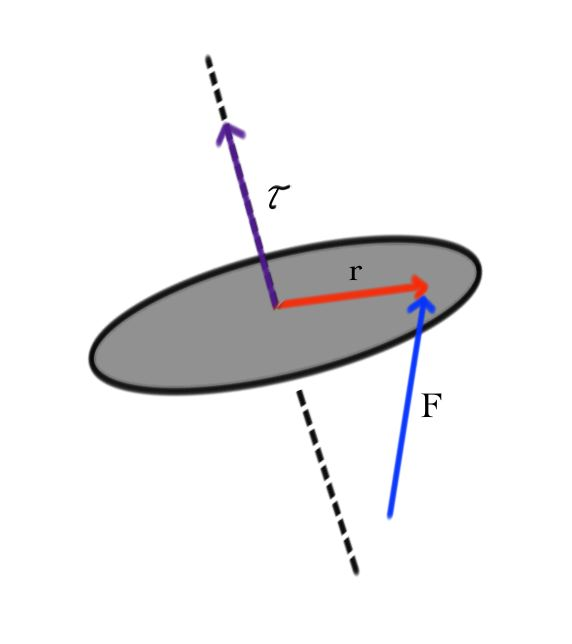
\includegraphics[alt={A disc spinning about its axis.  A vector F is the force applied to a point r away from the center of the disc.  This results in a torque τ=r×F.},scale=.27]{\whatIsPath/torque.jpg}
\end{center}
\vspace{-5mm}
Remember that the \index{Cross product}{\hypertarget{crossprod}{\itshape cross product}} of two $3$-vectors is given by 
\[\begin{pmatrix}x\\y\\z\end{pmatrix}\times\begin{pmatrix}x'\\y'\\z'\end{pmatrix}:=\begin{pmatrix}yz'-zy'\\zx'-xz'\\xy'-yx'\end{pmatrix}\, .\] Indeed, $3$-vectors are special, usually vectors  an only be added, not multiplied.

 Lets find the force $F$ (a vector)  one must apply to a wrench lying along the vector 
$r=\colvec{1 \\ 1\\ 0} \text{ft}$,
to produce a torque $\colvec{0\\0 \\ 1}$ft\,lb:

\begin{enumerate}
\item Find a solution by writing out this equation with $F=\colvec{ a \\[.5mm] b \\ c }$. 
(Hint: Guess and check that a solution with $a=0$ exists).
\item Add $\colvec{ 1 \\ 1 \\ 0 }$ to your solution and check that the result is a solution.
\item Give a  physics explanation of why there can be two solutions, and argue that there are, in fact, infinitely many solutions. 
\item \hypertarget{crossmat}{Set up a system} of three linear equations with the three components of $F$ as the variables which describes this situation. What happens if you try to solve these equations by substitution?
\end{enumerate}


\item
The function $P(t)$ gives gas prices (in units of dollars per gallon) as a function of  $t$ the year (in A.D. or C.E.), and $g(t)$ is the gas consumption rate measured in gallons per year by a %n average 
driver as a function of their age. 
The function $g$ is certainly different for different people. 
Assuming a lifetime is 100 years, what function gives the total amount spent on gas during the lifetime of an individual born in an arbitrary year $t$? Is the operator that maps $g$ to this function linear? \\
%, interpret the integrals 
%$\int_0^{100} P(2113-s) D(s) ds$ and $G(t)=\int_0^{100} P(t-s) D(s) ds$. 


%\item Let $M$ be a matrix and $u$ and $v$ vectors:
%
%$
%M=    \begin{pmatrix}
%      a             &b  \\
%      c             &d
%    \end{pmatrix},
%v = \colvec{ x \\ y }, u = \colvec{ w \\ z } 
%$.
%
%
%  \begin{enumerate}
%  \item \emph{Propose} a definition for $u+v$.
%  \item \emph{Check} that your definition obeys $Mv+Mu = M(u+v)$.
%  \end{enumerate}
%
%\phantomnewpage
%

\item The differential equation (DE) \[\frac{d}{dt} f=2f\] says that the rate of change of $f$ is proportional to $f$. It describes exponential growth because the exponential function 
\[f(t)=f(0)e^{2t}\] satisfies the DE for any number $f(0)$. The number 2 in the DE is called the constant of proportionality.  
A similar DE \[\frac{d}{dt}f=\frac{2}{t}f\] 
has a time-dependent ``constant of proportionality''.
\begin{enumerate}
\item Do you think that the second DE describes exponential growth? 
\item Write both DEs in the form $Df=0$ with $D$ a linear operator. 
\end{enumerate}

\item \label{Pablo} Pablo is a nutritionist who knows that oranges always have twice as much sugar as apples.  When considering the sugar intake of schoolchildren eating a barrel of fruit, he represents the barrel like so: 

\begin{tikzpicture}[alt={A graph with horizontal axis sugar and vertical axis fruit.},domain=0:4]
    \draw[very thin,color=gray] (-0.1,-1.1) grid (3.9,3.9);
    \draw[->] (-0.2,0) -- (4.2,0) node[right] {sugar};
    \draw[->] (0,-1.2) -- (0,4.2) node[above] {fruit};
    \draw[->] (0,0) -- (2,3) node[anchor=south east] {\scalebox{.75}{${ (s,f)}$}};
\end{tikzpicture}\hspace{3mm}
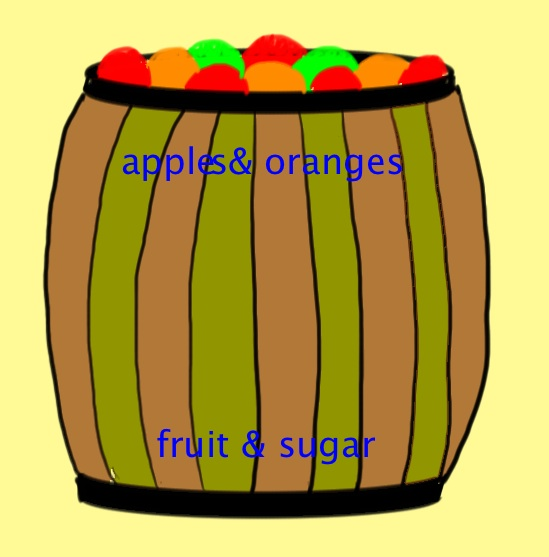
\includegraphics[alt={A barrel containing apples and oranges which have fruit and sugar.},scale=.38]{\whatIsPath/barrel2.jpg}


\emph{Find} a linear operator relating Pablo's representation to the ``everyday'' representation in terms of the number of apples and number of oranges.  Write your answer as a matrix.

\emph{Hint:} Let $\lambda$ represent the amount of sugar in each apple.

\Videoscriptlink{what_is_linear_algebra_hint.mp4}{Hint}{script_what_is_linear_algebra_hint}

%%%%%%%%%%%%%%%%%%%%%%%%%%%%%

\item\label{matmult} {\itshape Matrix Multiplication:}\index{Matrix multiplication} 
Let $M$ and $N$ be matrices
\[
M=    \begin{pmatrix}
      a             &b  \\
      c             &d
    \end{pmatrix}\, \mbox{ and }
    N=    \begin{pmatrix}
       e            &f  \\
       g            &h
    \end{pmatrix}\, ,
\]
and $v$ the vector
\[
v=    \begin{pmatrix}
      x               \\
      y             \end{pmatrix}\, .
\]
If we first apply $N$ and then $M$ to $v$ we obtain the vector $MNv$.\\
\begin{enumerate}
\item Show that the composition of matrices $MN$ is also a linear operator.\\
\item Write out the components of the matrix product $MN$ in terms of the components of $M$ and the components of $N$.
{\itshape Hint}: use the \hyperlink{ch1vecmult}{general rule} for multiplying a 2-vector by a 2$\times$2 matrix. 
\item Try to answer the following common question, ``Is there any sense in which these rules for matrix multiplication are unavoidable, or are they just a notation that could be replaced by some other notation?"
\item Generalize your multiplication rule to $3\times 3$ matrices.
\end{enumerate}

\item {\itshape \hypertarget{diagmat}{Diagonal} matrices:} A matrix $M$ can be thought of as an array of numbers $m^i_j$, known as matrix entries, or matrix components,  where $i$ and~$j$ index row and column numbers, respectively. Let 
\[
M=\begin{pmatrix}1&2\\3&4\end{pmatrix}=\big(m^i_j\big)\, .
\]
Compute $m^1_1$, $m^1_2$, $m^2_1$ and $m^2_2$. 

\noindent
The matrix entries $m^i_i$ whose row and column numbers are the same are called the {\itshape diagonal}
of $M$. Matrix entries $m^i_j$ with $i\neq j$ are called {\itshape off-diagonal}. How many diagonal entries does an $n\times n$ matrix have? How many off-diagonal 
entries does an $n\times n$ matrix have?

If all the off-diagonal entries of a matrix vanish, we say that the matrix is diagonal. Let
\[
D=\begin{pmatrix}\lambda&0\\0&\mu\end{pmatrix}\quad \mbox{and}\quad D'=\begin{pmatrix}\lambda'&0\\0&\mu'\end{pmatrix}\, .
\]
Are these matrices diagonal and why? Use the rule you found in problem~\ref{matmult} to compute
the matrix products $DD'$ and $D'D$. What do you observe? Do you think the same property holds for arbitrary matrices? What about products
where only one of the matrices is diagonal?\\

(p.s. Diagonal matrices play a special role in the study of matrices in linear algebra. Keep an eye out for this special role.)

\item \label{idprob} Find the linear operator that takes in vectors from $n$-space and gives out vectors from $n$-space in such a way that 
\begin{enumerate}
\item whatever you put in, you get exactly the same thing out as what you put in. Show that it is unique. Can you write this operator as a matrix? 
\item whatever you put in, you get exactly the same thing out as when you put something else in. Show that it is unique. Can you write this operator as a matrix? 
\end{enumerate}
{\itshape Hint:} To show something is unique, it is usually best to begin by pretending that it isn't, and then showing that this leads to a nonsensical conclusion. In mathspeak--{\itshape proof by contradiction}.

%\item Show that the order of columns in a matrix matters. 

\item \label{ch1rev} \hypertarget{Consider the set}{Consider the set} $S=\{*, \star, \# \}$. 
It contains just 3 elements, and has no  ordering; 
$\{*, \star, \# \}= \{ \# , \star, * \}$ {\itshape etc}. 
(In fact the same is true for  $\{1,2,3\}=\{2,3,1\}$ {\itshape etc}, although we could make this an {\itshape ordered set} using $3>2>1$.) 
\begin{enumext}[label=\roman*,wrap-label=(#1)]
\item \label{wasa} Invent a  function with domain $\{*, \star, \# \}$ and co\-domain~$\mathbb{R}$. (Remember that the {\itshape domain}\index{Domain} of a function is the set of all its allowed  inputs and the {\itshape codomain}\index{Codomain} (or {\itshape target space})\index{Target Space|seealso{Codomain}} is the set where the outputs can live. A function is specified by assigning exactly one codomain element to each element of the domain.)\\
\item Choose an ordering on  $\{*, \star, \# \}$, and then use it to write your function from part~(i) as a triple of numbers. \\
\item Choose a new ordering on $\{*, \star, \# \}$ and then write your function from part~(i) as a triple of numbers. \\
\item Your answers for parts (ii) and (iii) are different yet represent the same function -- explain!
\end{enumext}

%In fact, the point of this problem is that order doesn't matter. 
%We can explicitly define a function $f$ on this set by explicitly specifying 
%\[f(\star)=7, f(*)=3, f(\#)=-2\]. 


%Our students do not need to think about non-associative algebras -cherney
%%%%%%%%%%%
%Next recall that multiplication of ordinary numbers is associative, namely the order of brackets
%does not matter: $(xy)z=x(yz)$. Let us try to demand the same property for matrices and vectors,
%that is
%\[
%M(Nv) = (MN) v\, .
%\] 
%We need to be careful reading this equation because $Nv$ is a vector and so is $M(Nv)$.
%Therefore the right hand side, $(MN) v$ should also be a vector. This means that 
%%%%%%%%%%%%%%%
%$MN$
%must be a matrix; in fact it is the matrix obtained by multiplying the matrices $M$ and $N$.
% Use your result for $M(Nv)$ to find the matrix $MN$.

%Gaussian elimination is next chapter! 
%\item 
%    There are methods for solving linear systems other 
%    than Gauss' method.
%    One often taught in high school is to solve one of the 
%    equations for a variable, then substitute the resulting expression into
%    other equations.
%    That step is repeated until there is an equation with only one
%    variable.
%    From that, the first number in the solution is derived, and then 
%    back-substitution can be done.
%    This method takes longer than Gauss' method, since it involves
%    more arithmetic operations, and is also more
%    likely to lead to errors.
%    To illustrate how it can lead to wrong conclusions, we will use the system 
%    \begin{equation*}
%      \begin{linsys}{2}
%            x  &+  &3y  &=  &1  \\
%            2x  &+  &y   &=  &-3 \\
%            2x  &+  &2y  &=  &0  
%      \end{linsys}
%    \end{equation*}
%
%    \begin{enumerate}
%      \item Solve the first equation for $x$ and 
%        substitute that expression into the second equation.
%        Find the resulting $y$.
%      \item Again solve the first equation for $x$, 
%        but this time substitute that expression into the third equation.
%        Find this $y$.
%    \end{enumerate}
%    What extra step must a user of this method take to avoid 
%    erroneously concluding a system has a solution?
%
\phantomnewpage

\end{enumerate}

%\phantomnewpage
